% THIS IS SIGPROC-SP.TEX - VERSION 3.1
% WORKS WITH V3.2SP OF ACM_PROC_ARTICLE-SP.CLS
% APRIL 2009
%
% It is an example file showing how to use the 'acm_proc_article-sp.cls' V3.2SP
% LaTeX2e document class file for Conference Proceedings submissions.
% ----------------------------------------------------------------------------------------------------------------
% This .tex file (and associated .cls V3.2SP) *DOES NOT* produce:
%       1) The Permission Statement
%       2) The Conference (location) Info information
%       3) The Copyright Line with ACM data
%       4) Page numbering
% ---------------------------------------------------------------------------------------------------------------
% It is an example which *does* use the .bib file (from which the .bbl file
% is produced).
% REMEMBER HOWEVER: After having produced the .bbl file,
% and prior to final submission,
% you need to 'insert'  your .bbl file into your source .tex file so as to provide
% ONE 'self-contained' source file.
%
% Questions regarding SIGS should be sent to
% Adrienne Griscti ---> griscti@acm.org
%
% Questions/suggestions regarding the guidelines, .tex and .cls files, etc. to
% Gerald Murray ---> murray@hq.acm.org
%
% For tracking purposes - this is V3.1SP - APRIL 2009

\documentclass{acm_proc_article-sp}
\usepackage{amsmath,amssymb,latexsym,graphicx,url}
\begin{document}


%\title{A Sample {\ttlit ACM} SIG Proceedings Paper in LaTeX
%Format\titlenote{(Does NOT produce the permission block, copyright information nor page numbering). For use with ACM\_PROC\_ARTICLE-SP.CLS. Supported by ACM.}}
\title{ Spiking Neural P system without delay simulator implementation using GPGPUs }
%\subtitle{[Extended Abstract]
%\titlenote{A full version of this paper is available as
%\textit{Author's Guide to Preparing ACM SIG Proceedings Using
%\LaTeX$2_\epsilon$\ and BibTeX} at
%\texttt{www.acm.org/eaddress.htm}}}
%
% You need the command \numberofauthors to handle the 'placement
% and alignment' of the authors beneath the title.
%
% For aesthetic reasons, we recommend 'three authors at a time'
% i.e. three 'name/affiliation blocks' be placed beneath the title.
%
% NOTE: You are NOT restricted in how many 'rows' of
% "name/affiliations" may appear. We just ask that you restrict
% the number of 'columns' to three.
%
% Because of the available 'opening page real-estate'
% we ask you to refrain from putting more than six authors
% (two rows with three columns) beneath the article title.
% More than six makes the first-page appear very cluttered indeed.
%
% Use the \alignauthor commands to handle the names
% and affiliations for an 'aesthetic maximum' of six authors.
% Add names, affiliations, addresses for
% the seventh etc. author(s) as the argument for the
% \additionalauthors command.
% These 'additional authors' will be output/set for you
% without further effort on your part as the last section in
% the body of your article BEFORE References or any Appendices.

\numberofauthors{2} %  in this sample file, there are a *total*
% of EIGHT authors. SIX appear on the 'first-page' (for formatting
% reasons) and the remaining two appear in the \additionalauthors section.
%
\author{
% You can go ahead and credit any number of authors here,
% e.g. one 'row of three' or two rows (consisting of one row of three
% and a second row of one, two or three).
%
% The command \alignauthor (no curly braces needed) should
% precede each author name, affiliation/snail-mail address and
% e-mail address. Additionally, tag each line of
% affiliation/address with \affaddr, and tag the
% e-mail address with \email.
%
% 1st. author
\alignauthor
Francis Cabarle \\
       \affaddr{ Algorithms and Complexity Laboratory }\\
       \affaddr{ Department of Computer Science }\\
       \affaddr{ University of the Philippines Diliman }\\
       \email{ fccabarle@up.edu.ph  }
% 2nd. author
\alignauthor
Henry Adorna \\
       \affaddr{ Algorithms and Complexity Laboratory }\\
       \affaddr{ Department of Computer Science }\\
       \affaddr{ University of the Philippines Diliman }\\
       \email{hnadorna@dcs.upd.edu.ph}
%\and  % use '\and' if you need 'another row' of author names
}
% There's nothing stopping you putting the seventh, eighth, etc.
% author on the opening page (as the 'third row') but we ask,
% for aesthetic reasons that you place these 'additional authors'
% in the \additional authors block, viz.

%\additionalauthors{Additional authors: John Smith (The Th{\o}rv{\"a}ld Group,
%email: {\texttt{jsmith@affiliation.org}}) and Julius P.~Kumquat
%(The Kumquat Consortium, email: {\texttt{jpkumquat@consortium.net}}).}
%\date{30 July 1999}

% Just remember to make sure that the TOTAL number of authors
% is the number that will appear on the first page PLUS the
% number that will appear in the \additionalauthors section.

\maketitle
\begin{abstract}

This paper presents a parallel simulator for a type of P system known as spiking neural P system (SNP system) using general purpose graphics processing units (GPGPUs). GPGPUs, unlike the more conventional and general purpose, multi-core CPUs, are used for parallelizable problems due to their architectural optimization for parallel computations.

Membrane computing or P systems on the other hand, are cell-inspired computational models which compute in a maximally parallel and non-deterministic manner. SNP systems, w/c compute via time separated spikes and whose inspiration was taken from the way neurons operate in living organisms, have been represented as matrices.

The matrix representation of SNP systems provides a crucial step into their simulation on parallel devices such as GPGPUs. Simulating the highly parallel nature of SNP systems necessitates the use of hardware intended for parallel computations. The simulator algorithms, design considerations, and implementation are presented. Finally, simulation results, observations, and analyses using an SNP system that generates all numbers in \{$\mathbb N$ - $1$\} are discussed.

\end{abstract}

% A category with the (minimum) three required fields
%\category{H.4}{Information Systems Applications}{Miscellaneous}
%A category including the fourth, optional field follows...
%\category{D.2.8}{Software Engineering}{Metrics}[complexity measures, performance measures]

%\terms{Theory}

\keywords{ Membrane computing, Parallel computing, GPU computing  } % NOT required for Proceedings

\section{Introduction}

\subsection{Parallel computing: Via graphics processing units (GPUs)}
The trend for massively parallel computation is moving from the more common multi-core CPUs towards GPGPUs for several significant reasons \cite{cudabook}\cite{cudaguide}. One important reason for such a trend in recent years include the low consumption in terms of power of GPGPUs compared to setting up machines and infrastructure which will utilize multiple CPUs in order to obtain the same level of parallelization and performance\cite{cudapage}. Another more important reason is that GPGPUs are architectured for massively parallel computations since unlike the architectures of most general purpose CPUs, a large part of GPGPUs are devoted for arithmetic operations and not on control and caching \cite{cudabook}\cite{cudaguide}. Arithmetic operations are at the heart of many basic operations as well as scientific computations, and these are performed with  larger speedups when done in parallel, by GPGPUs over CPUs. 

\subsection{Paralel computing: Via Membranes}
Membrane computing or its more specific counterpart, a P system, are Turing complete computing models that perform computations nondeterministically, exhausting all possible  computations at any given time. This type of unconventional model of computation was introduced by Gheorghe P\u aun in 1998 and takes inspiration, similar to other members of natural computing, from nature\cite{introtomem}\cite{ppage}. Specifically, P systems try to mimic the constitution and dynamics of the living cell: the multitude of elements inside it, and their interactions within themselves and their environment, or outside the cell's skin membrane.

SN P systems differ from other types of P systems precisely because they are mono-membranar and only use one type of object in its computation. These characteristics, among others, are meant to capture the workings of a special type of cell known as the neuron. Neurons, such as those in the human brain, communicate or 'compute' by sending indistinct electro-chemical  signals more commonly known as spikes. Information is then communicated and encoded not by the spikes themselves, since the spikes are unrecognizable from one another, by means of time duration as well as the number of spikes sent/received from one neuron to another, oftentimes under a certain time interval\cite{snp}. The time duration between two spikes, or several successive spikes, transmit information from one cell to another.  

It has been shown that SN P systems, given their nature, are representable by matrices\cite{snpbrain}\cite{snpmat}. This representation allows design and implementation of an SN P system simulator using parallel computing machines such as GPGPUs. 

\subsection{Simulating SNP systems in GPGPUs}
Matrix operations and their algorithms have been studied and efficiently implemented in GPGPUs \cite{matrixgpu1}\cite{matrixgpu2}. Thus the matrix representation of SNP systems bridges the gap between the highly theoretical yet still computationally powerful SNP systems and the applicative and more tangible GPGPUs, via an SNP system simulator. The design of the simulator, including the algorithms deviced, architectural considerations, are then implemented using a particular type of GPGPU, namely NVIDIA CUDA (compute unified device architecture). NVIDIA CUDA extends the widely known ANSI C programming language and makes parallel computations, via GPGPUs manufactured by NVIDIA.

This paper starts out by introducing and defining the type of SNP system that will be simulated. Afterwards the NVIDIA CUDA model and architecture are discussed, baring the scalability and parallelization CUDA offers. Next, the design of the simulator, constraints and considerations, as well as the details of the algorithms used to realize the SNP system are discussed. The simulation results are presented next, as well as observations and analysis of these results. The paper ends by providing the conclusions and future work.

%MENTION matrix implementation on parallel/GPU systems + citations (DONE)

%MENTION overview of paper + contributions BRIEFLY (DONE)


\section{Spiking neural p systems}

\subsection{Computing with SNP systems}
The type of SNP systems focused on by this paper are those without delays i.e. those that spike or transmit signals the moment they are able to do so \cite{snpbrain}\cite{snpmat}. A variant, which allows for delays before a neuron produces a spike, are also available \cite{snp}. An SNP system without delay is of the form:

%MODIFY the following defitions or CITE them instead

\begin{definition} 
$$\Pi=(O,\sigma_1,\ldots, \sigma_m, syn, in, out),$$
where:
\begin{enumerate}
\item[1.] $O=\{a\}$ is the alphabet made up of only one object, the system spike $a$.

\item[2.] $\sigma_1,\ldots, \sigma_m$ are $m$ number of neurons of the form
$$\sigma_{i}=(n_i, R_i),1\leq i\leq m,$$
where:
\begin{enumerate}
\item[a)] $n_i\geq 0$ gives the initial number of $a$s i.e. spikes contained in neuron $\sigma_i$
\item[b)] $R_i$ is a finite set of rules of with two forms:
\begin{enumerate}
\item[(b-1)]$E/a^c \rightarrow a$, are known as \textit{Spiking rules}, where $E$ is a regular expression
over $a$, and $c\geq 1$, such that $c\geq 1$. 
\item[(b-2)]$a^s\rightarrow \lambda$, are known as \textit{Forgetting rules}, for $s\geq 1$, such that for each rule $E/a^c\rightarrow a$ of type (b-1) from $R_i$, $a^s\notin L(E)$. 
\end{enumerate}
\end{enumerate}
\item[3.] $syn= \{ (i,j)\, |\, 1\leq i,j \leq m, \, i\neq j\, \}$ are the synapses i.e. connection between neurons.

\item[4.] $in, out\in \{1,2,\ldots, m\}$ are the input and output neurons, respectively.
\end{enumerate}

\end{definition}

Furthermore, rules of type (b-1) are applied if $\sigma_i$ contains $k$
spikes, $a^k \in L(E)$ and $k \geq c$. Using this type of rule uses up
or consumes k spikes from the neuron, producing a spike to
each of the neurons connected to it via a forward pointing arrow i.e. away from the neuron. In this manner, for rules of type (b-2)
if $\sigma_i$ contains $s$ spikes, then $s$ spikes are forgotten or
removed once the rule is used. Rules of type (b-1) can be
simplified with the notation

\begin{definition}
\begin{enumerate}
\begin{enumerate}
\begin{enumerate}
\item[(b-3)]$a^k \rightarrow a$
\end{enumerate}
\end{enumerate}
\end{enumerate}
\end{definition}
%b-3) a → a

where the regular expression $E = a^k$, again consuming $k$ spikes and producing a spike.

The non-determinism of SNP systems comes with the fact
that more than one rule of the several types are applicable at
a given time, given enough spikes. The rule to be used is
chosen non-deterministically in the neuron. However, only
one rule can be applied or used at a given time \cite{snp}\cite{snpbrain}\cite{snpmat}. The
neurons in an SN P system operate in parallel and in unison,
under a global clock \cite{snp}. For Figure \ref{snp_ex} no input neuron is present,
but neuron 3 is the output neuron, hence the arrow pointing
towards the environment, outside the SNP system. The SNP system in Figure \ref{snp_ex} is a 3 neuron system whose neurons are labeled (neuron/$\sigma_1$ to 3) and whose rules have a total system ordering from (1) to (5)


	\begin{figure}
		\centering
		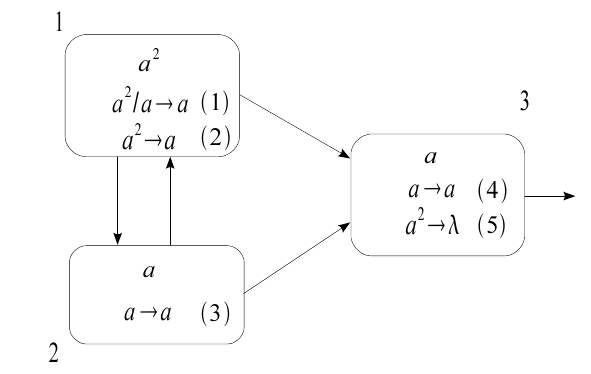
\includegraphics[scale=.5]{snp-img.png} 
%		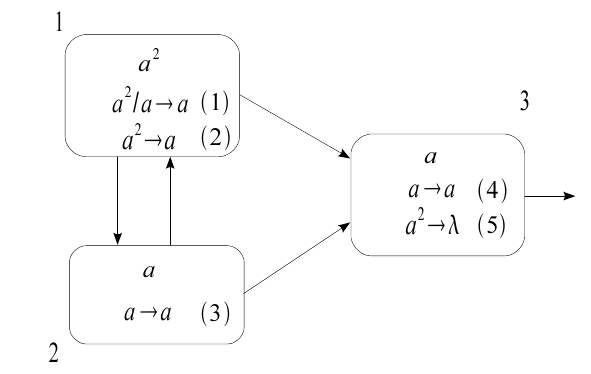
\includegraphics[height=2in, width=2.5in]{snp-img.PNG}
		\caption{An SNP P system $\Pi$, generating all numbers in \{$\mathbb N$ - $1$\}, from \cite{snpmat}.}
		\label{snp_ex}
	\end{figure}
%$<$

%cite references for figures used!!!

%\subsection{Type Changes and {\subsecit Special} Characters}
%of\footnote{A fourth, and last, footnote.}

%\subsection{Math Equations}
%You may want to display math equations in three distinct styles: the three are discussed in the next sections.

%\subsubsection{Inline (In-text) Equations}
%A formula that appears in the running text is called an

%\subsubsection{Display Equations}
%A numbered display equation -- one set off by vertical space



\subsection{Matrix representation of SNP systems}
A matrix representation of an SN P system makes use of the
following vectors and matrix definitions \cite{snpbrain}\cite{snpmat} . It is important to note that, just as in Figure \ref{snp_ex}, a total ordering of rules is in
order.

\textit{Configuration vector} $C_k$ is the vector containing all spikes in every neuron on the $kth$ computation step/time, where $C_0$ is the initial vector containing all spikes in the system at the beginning of the computation. For $\Pi$ (in Figure \ref{snp_ex} ) the initial configuration vector is $C_0 = < 2, 1, 1 >$.

\textit{Spiking vector} which shows, at a given configuration $C_k$, if a
rule is applicable (has value 1) or not (has value 0 instead). For $\Pi$ we have the
spiking vector $S_k = < 1, 0, 1, 1, 0 >$ given $C_0$.
Note that a 2nd spiking vector, $S_k = < 1, 0, 1, 1, 0 >$, is
possible if we use rule (2) over rule (1) instead (but not both
at the same time, hence we cannot have a vector equal to
< 1, 1, 1, 1, 0> ).

\textit{Spiking transition matrix} $M_{\Pi}$ is a matrix comprised of $a_i_j$
elements where $a_i_j$ is given as

\begin{definition}\label{defi-snp-mat}
$$
a_{ij} = \left\{
\begin{array}{rl}
-c, &\mbox{if rule $r_i$ is in $\sigma_j$ and it is applied consuming $c$ spikes;} \\
 p, &\mbox{if rule $r_i$ is in $\sigma_s$ ($s\neq j$ and $(s,j)\in syn$)} \\
 & \mbox{and it is applied producing $p$ spikes in total;}\\
 0, &\mbox{if rule $r_i$ is in $\sigma_s$ ($s\neq j$ and $(s,j)\notin syn$).}
    \end{array}
\right.
$$
\end{definition}


\subsection{Citations}
Citations to articles \cite{bowman:reasoning, clark:pct, braams:babel, herlihy:methodology},
conference
proceedings \cite{clark:pct} or books \cite{salas:calculus, Lamport:LaTeX} listed
in the Bibliography section of your
article will occur throughout the text of your article.
You should use BibTeX to automatically produce this bibliography;
you simply need to insert one of several citation commands with
a key of the item cited in the proper location in
the \texttt{.tex} file \cite{Lamport:LaTeX}.
The key is a short reference you invent to uniquely
identify each work; in this sample document, the key is
the first author's surname and a
word from the title.  This identifying key is included
with each item in the \texttt{.bib} file for your article.

The details of the construction of the \texttt{.bib} file
are beyond the scope of this sample document, but more
information can be found in the \textit{Author's Guide},
and exhaustive details in the \textit{\LaTeX\ User's
Guide}\cite{Lamport:LaTeX}.

This article shows only the plainest form
of the citation command, using \texttt{{\char'134}cite}.
This is what is stipulated in the SIGS style specifications.
No other citation format is endorsed.

\subsection{Tables}
Because tables cannot be split across pages, the best
placement for them is typically the top of the page
nearest their initial cite.  To
ensure this proper ``floating'' placement of tables, use the
environment \textbf{table} to enclose the table's contents and
the table caption.  The contents of the table itself must go
in the \textbf{tabular} environment, to
be aligned properly in rows and columns, with the desired
horizontal and vertical rules.  Again, detailed instructions
on \textbf{tabular} material
is found in the \textit{\LaTeX\ User's Guide}.

Immediately following this sentence is the point at which
Table 1 is included in the input file; compare the
placement of the table here with the table in the printed
dvi output of this document.


To set a wider table, which takes up the whole width of
the page's live area, use the environment
\textbf{table*} to enclose the table's contents and
the table caption.  As with a single-column table, this wide
table will ``float" to a location deemed more desirable.
Immediately following this sentence is the point at which
Table 2 is included in the input file; again, it is
instructive to compare the placement of the
table here with the table in the printed dvi
output of this document.


\begin{table*}
\centering
\caption{Some Typical Commands}
\begin{tabular}{|c|c|l|} \hline
Command&A Number&Comments\\ \hline
\texttt{{\char'134}alignauthor} & 100& Author alignment\\ \hline
\texttt{{\char'134}numberofauthors}& 200& Author enumeration\\ \hline
\texttt{{\char'134}table}& 300 & For tables\\ \hline
\texttt{{\char'134}table*}& 400& For wider tables\\ \hline\end{tabular}
\end{table*}
% end the environment with {table*}, NOTE not {table}!

\subsection{Figures}
Like tables, figures cannot be split across pages; the
best placement for them
is typically the top or the bottom of the page nearest
their initial cite.  To ensure this proper ``floating'' placement
of figures, use the environment
\textbf{figure} to enclose the figure and its caption.

This sample document contains examples of \textbf{.eps}
and \textbf{.ps} files to be displayable with \LaTeX.  More
details on each of these is found in the \textit{Author's Guide}.

\begin{figure}
\centering
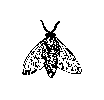
\epsfig{file=fly.eps}
\caption{A sample black and white graphic (.eps format).}
\end{figure}

\begin{figure}
\centering
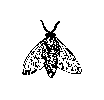
\epsfig{file=fly.eps, height=1in, width=1in}
\caption{A sample black and white graphic (.eps format)
that has been resized with the \texttt{epsfig} command.}
\end{figure}


As was the case with tables, you may want a figure
that spans two columns.  To do this, and still to
ensure proper ``floating'' placement of tables, use the environment
\textbf{figure*} to enclose the figure and its caption.

Note that either {\textbf{.ps}} or {\textbf{.eps}} formats are
used; use
the \texttt{{\char'134}epsfig} or \texttt{{\char'134}psfig}
commands as appropriate for the different file types.

\subsection{Theorem-like Constructs}
Other common constructs that may occur in your article are
the forms for logical constructs like theorems, axioms,
corollaries and proofs.  There are
two forms, one produced by the
command \texttt{{\char'134}newtheorem} and the
other by the command \texttt{{\char'134}newdef}; perhaps
the clearest and easiest way to distinguish them is
to compare the two in the output of this sample document:

This uses the \textbf{theorem} environment, created by
the\linebreak\texttt{{\char'134}newtheorem} command:
\newtheorem{theorem}{Theorem}
\begin{theorem}
Let $f$ be continuous on $[a,b]$.  If $G$ is
an antiderivative for $f$ on $[a,b]$, then
\begin{displaymath}\int^b_af(t)dt = G(b) - G(a).\end{displaymath}
\end{theorem}

The other uses the \textbf{definition} environment, created
by the \texttt{{\char'134}newdef} command:
\newdef{definition}{Definition}
\begin{definition}
If $z$ is irrational, then by $e^z$ we mean the
unique number which has
logarithm $z$: \begin{displaymath}{\log e^z = z}\end{displaymath}
\end{definition}

\begin{figure}
\centering

\psfig{file=rosette.ps, height=1in, width=1in,}
\caption{A sample black and white graphic (.ps format) that has
been resized with the \texttt{psfig} command.}
\end{figure}

Two lists of constructs that use one of these
forms is given in the
\textit{Author's  Guidelines}.

\begin{figure*}
\centering
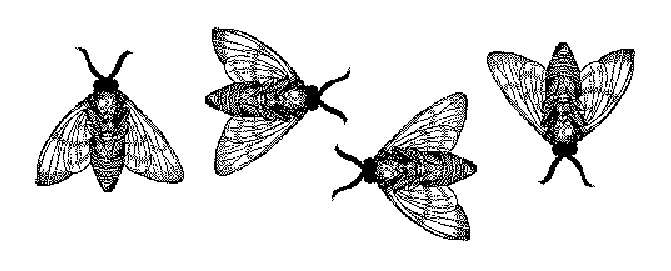
\epsfig{file=flies.eps}
\caption{A sample black and white graphic (.eps format)
that needs to span two columns of text.}
\end{figure*}
and don't forget to end the environment with
{figure*}, not {figure}!
 
There is one other similar construct environment, which is
already set up
for you; i.e. you must \textit{not} use
a \texttt{{\char'134}newdef} command to
create it: the \textbf{proof} environment.  Here
is a example of its use:
\begin{proof}
Suppose on the contrary there exists a real number $L$ such that
\begin{displaymath}
\lim_{x\rightarrow\infty} \frac{f(x)}{g(x)} = L.
\end{displaymath}
Then
\begin{displaymath}
l=\lim_{x\rightarrow c} f(x)
= \lim_{x\rightarrow c}
\left[ g{x} \cdot \frac{f(x)}{g(x)} \right ]
= \lim_{x\rightarrow c} g(x) \cdot \lim_{x\rightarrow c}
\frac{f(x)}{g(x)} = 0\cdot L = 0,
\end{displaymath}
which contradicts our assumption that $l\neq 0$.
\end{proof}

Complete rules about using these environments and using the
two different creation commands are in the
\textit{Author's Guide}; please consult it for more
detailed instructions.  If you need to use another construct,
not listed therein, which you want to have the same
formatting as the Theorem
or the Definition\cite{salas:calculus} shown above,
use the \texttt{{\char'134}newtheorem} or the
\texttt{{\char'134}newdef} command,
respectively, to create it.

\subsection*{A {\secit Caveat} for the \TeX\ Expert}
Because you have just been given permission to
use the \texttt{{\char'134}newdef} command to create a
new form, you might think you can
use \TeX's \texttt{{\char'134}def} to create a
new command: \textit{Please refrain from doing this!}
Remember that your \LaTeX\ source code is primarily intended
to create camera-ready copy, but may be converted
to other forms -- e.g. HTML. If you inadvertently omit
some or all of the \texttt{{\char'134}def}s recompilation will
be, to say the least, problematic.

\section{Conclusions and future work}
Using a highly parallel computing device such as a GPGPU,
particularly NVIDIA CUDA, an SNP system simulator was
successfully designed and implemented. The use of a high
level programming language such as Python for host tasks,
mainly for logic and string representation and manipulation
of values (vector/matrix elements) provided the necessary
expressivity to implement the algorithms created to produce
and exhaust all possible and valid configuration and spiking
vectors. For the device tasks, CUDA C allowed the
manipulation of the NVIDIA CUDA enabled GPGPU which
took care of repetitive and highly parallel computations
(addition and multiplication essentially).

Future versions of the SNP system simulator will focus on
several improvements. These improvements include the use
of an algorithm for matrix computations without requiring
the input matrix to be turned into a square matrix (this is
currently handled by the simulator by padding zeros to an
otherwise non-square matrix input). Another improvement
would be the simulation of systems not of the form b-3).
Byte-compiling the Python/host part of the code to improve
performance as well as metrics to further enhance and
measure execution time are desirable as well. Finally, deeper
understanding of the CUDA architecture, such as inter-
thread/block communication, for extremely large systems
with equally large matrices, is required. These
improvements as well as the current version of the simulator
should also be run in a machine with higher versions of
GPGPUs running NVIDIA CUDA.
%ADD simulation in larger CUDA systems

%\end{document}  % This is where a 'short' article might terminate

%ACKNOWLEDGMENTS are optional
\section{ Acknowledgments }
The authors are supported by the \textit{ERDT Project}. They also wish to acknowledge the \textit{Algorithms and Complexity laboratory} of \textit{UP Diliman Department of Computer Science} for the use of Apple iMacs with NVIDIA CUDA enabled GPUs, which provided the proper environment for the simulations, their development, design and tests.

%HOW to acknowledge Mr. Miguel del-Amor?

%and the \textbf{.cls} and \textbf{.tex} files that it describes.

%
% The following two commands are all you need in the
% initial runs of your .tex file to
% produce the bibliography for the citations in your paper.
%\bibliographystyle{abbrv}
%\bibliography{sigproc}  % sigproc.bib is the name of the Bibliography in this case

\begin{thebibliography}{9999}

%MUST learn how to use bibtex

%\bibitem{adorna} H. Adorna, Gh. P\u aun, M. P\'{e}rez-Jim\'{e}nez : On Communication Complexity in Evolution-Communication P Systems, {\it Proc. Eighth Brainstorming Week on Membrane Computing, Sevilla, February 1-5, 2010}

%journal citation
\bibitem{snp} M. Ionescu, Gh. P\u aun, T. Yokomori, ``Spiking Neural P Systems'', {\it Journal Fundamenta Informaticae  }, vol. 71, issue 2,3 pp. 279-308, Feb. 2006.

%proceedings/brainstorming citation
\bibitem{snpbrain} X. Zeng, H. Adorna, M. A. Martinez-del-Amor, L. Pan, ``When Matrices Meet Brains'', {\it Proceedings of the Eighth Brainstorming Week on Membrane Computing }, Sevilla, Spain, Feb. 2010.

%conference citation
\bibitem{snpmat} X. Zeng, H. Adorna, M. A. Martinez-del-Amor, L. Pan, M. P\'{e}rez-Jim\'{e}nez, ``Matrix Representation of Spiking Neural P Systems'', {\it 11th International Conference on Membrane Computing }, Jena, Germany, Aug. 2010.

%\bibitem{backward} M.A. Gutierrez-Naranjo, M.J. P\'{e}rez-Jim\'{e}nez: Computing Backwards with P Systems, $WMC10$, Curtea de Arge\c s, Romania, (2009), 282-295.

\bibitem{introtomem} Gh. P\u aun, G. Ciobanu, M. P\'{e}rez-Jim\'{e}nez (Eds), {\it ``Applications of Membrane Computing'' }, Natural Computing Series, Springer, 2006.

%website citation (IEEE format)
\bibitem{ppage} P systems resource website. (2010, Jan) [Online]. Available: {\tt www.ppage.psystems.eu}.

\bibitem{sat} J. Cecilia, J. Garcia, G. Guerrero, M. Martinez-del-Amor, I. Perez-Jurtado, M.J. P\'{e}rez-Jim\'{e}nez, ``Simulating a P system based efficient solution to SAT by using GPUs'', {\it Journal of Logic and Algebraic Programming }, Vol 79, issue 6, pp. 317-325, Apr. 2010.

%book citation (IEEE format)
\bibitem{cudabook} D. Kirk, W. Hwu, {\it ``Programming Massively Parallel Processors: A Hands On Approach'' }, 1st ed. MA, USA: Morgan Kaufmann, 2010.

\bibitem{cudaguide} NVIDIA corporation, {\it ``NVIDIA CUDA C programming guide'' }, version 3.0, CA, USA: NVIDIA, 2010.

\bibitem{cudapage} NVIDIA CUDA developers resources page: tools, presentations, whitepapers. (2010, Jan) [Online]. Available: {\tt http://developer.nvidia.com/page/home.html }.

%ADD matrix on parallel computers book citation

%William Schmeister. 2006. Review of "Algorithms: Sequential, Parallel, and Distributed by Kenneth A. Berman and Jerome L. Paul", Thomson Course Technology, 2005. SIGACT News 37, 2 (June 2006), 17-22. DOI=10.1145/1140612.1140616 http://doi.acm.org/10.1145/1140612.1140616

%ADD citation to figures used!!

\bibitem{matrixgpu1} V. Volkov, J. Demmel, ``Benchmarking GPUs to tune dense linear algebra'', {\it Proceedings of the 2008 ACM/IEEE conference on Supercomputing}, NJ, USA, 2008.

\bibitem{matrixgpu2} K. Fatahalian, J. Sugerman, P. Hanrahan, ``Understanding the efficiency of GPU algorithms for matrix-matrix multiplication'', {\it In Proceedings of the ACM SIGGRAPH/EUROGRAPHICS conference on Graphics hardware (HWWS '04) }, ACM, NY, USA, pp. 133-137, 2004

\end{thebibliography}


% You must have a proper ".bib" file
%  and remember to run:
% latex bibtex latex latex
% to resolve all references
%
% ACM needs 'a single self-contained file'!
%
%APPENDICES are optional
%\balancecolumns

%removed appendices

% That's all folks!
\end{document}
